\documentclass[]{book}
\usepackage{lmodern}
\usepackage{amssymb,amsmath}
\usepackage{ifxetex,ifluatex}
\usepackage{fixltx2e} % provides \textsubscript
\ifnum 0\ifxetex 1\fi\ifluatex 1\fi=0 % if pdftex
  \usepackage[T1]{fontenc}
  \usepackage[utf8]{inputenc}
\else % if luatex or xelatex
  \ifxetex
    \usepackage{mathspec}
  \else
    \usepackage{fontspec}
  \fi
  \defaultfontfeatures{Ligatures=TeX,Scale=MatchLowercase}
\fi
% use upquote if available, for straight quotes in verbatim environments
\IfFileExists{upquote.sty}{\usepackage{upquote}}{}
% use microtype if available
\IfFileExists{microtype.sty}{%
\usepackage{microtype}
\UseMicrotypeSet[protrusion]{basicmath} % disable protrusion for tt fonts
}{}
\usepackage[margin=1in]{geometry}
\usepackage{hyperref}
\hypersetup{unicode=true,
            pdftitle={Encyclopedia of Quantitative Methods in R, vol.~0: Setting up Your Computer},
            pdfauthor={Sarah Schwartz \& Tyson Barrett},
            pdfborder={0 0 0},
            breaklinks=true}
\urlstyle{same}  % don't use monospace font for urls
\usepackage{natbib}
\bibliographystyle{apalike}
\usepackage{longtable,booktabs}
\usepackage{graphicx,grffile}
\makeatletter
\def\maxwidth{\ifdim\Gin@nat@width>\linewidth\linewidth\else\Gin@nat@width\fi}
\def\maxheight{\ifdim\Gin@nat@height>\textheight\textheight\else\Gin@nat@height\fi}
\makeatother
% Scale images if necessary, so that they will not overflow the page
% margins by default, and it is still possible to overwrite the defaults
% using explicit options in \includegraphics[width, height, ...]{}
\setkeys{Gin}{width=\maxwidth,height=\maxheight,keepaspectratio}
\IfFileExists{parskip.sty}{%
\usepackage{parskip}
}{% else
\setlength{\parindent}{0pt}
\setlength{\parskip}{6pt plus 2pt minus 1pt}
}
\setlength{\emergencystretch}{3em}  % prevent overfull lines
\providecommand{\tightlist}{%
  \setlength{\itemsep}{0pt}\setlength{\parskip}{0pt}}
\setcounter{secnumdepth}{5}
% Redefines (sub)paragraphs to behave more like sections
\ifx\paragraph\undefined\else
\let\oldparagraph\paragraph
\renewcommand{\paragraph}[1]{\oldparagraph{#1}\mbox{}}
\fi
\ifx\subparagraph\undefined\else
\let\oldsubparagraph\subparagraph
\renewcommand{\subparagraph}[1]{\oldsubparagraph{#1}\mbox{}}
\fi

%%% Use protect on footnotes to avoid problems with footnotes in titles
\let\rmarkdownfootnote\footnote%
\def\footnote{\protect\rmarkdownfootnote}

%%% Change title format to be more compact
\usepackage{titling}

% Create subtitle command for use in maketitle
\newcommand{\subtitle}[1]{
  \posttitle{
    \begin{center}\large#1\end{center}
    }
}

\setlength{\droptitle}{-2em}

  \title{Encyclopedia of Quantitative Methods in R, vol.~0: Setting up Your
Computer}
    \pretitle{\vspace{\droptitle}\centering\huge}
  \posttitle{\par}
    \author{Sarah Schwartz \& Tyson Barrett}
    \preauthor{\centering\large\emph}
  \postauthor{\par}
      \predate{\centering\large\emph}
  \postdate{\par}
    \date{Last updated: 2018-08-15}

\usepackage{booktabs}
\usepackage{amsthm}
\makeatletter
\def\thm@space@setup{%
  \thm@preskip=8pt plus 2pt minus 4pt
  \thm@postskip=\thm@preskip
}
\makeatother

\begin{document}
\maketitle

{
\setcounter{tocdepth}{1}
\tableofcontents
}
\chapter*{Welcome}\label{welcome}
\addcontentsline{toc}{chapter}{Welcome}

\begin{figure}
\centering
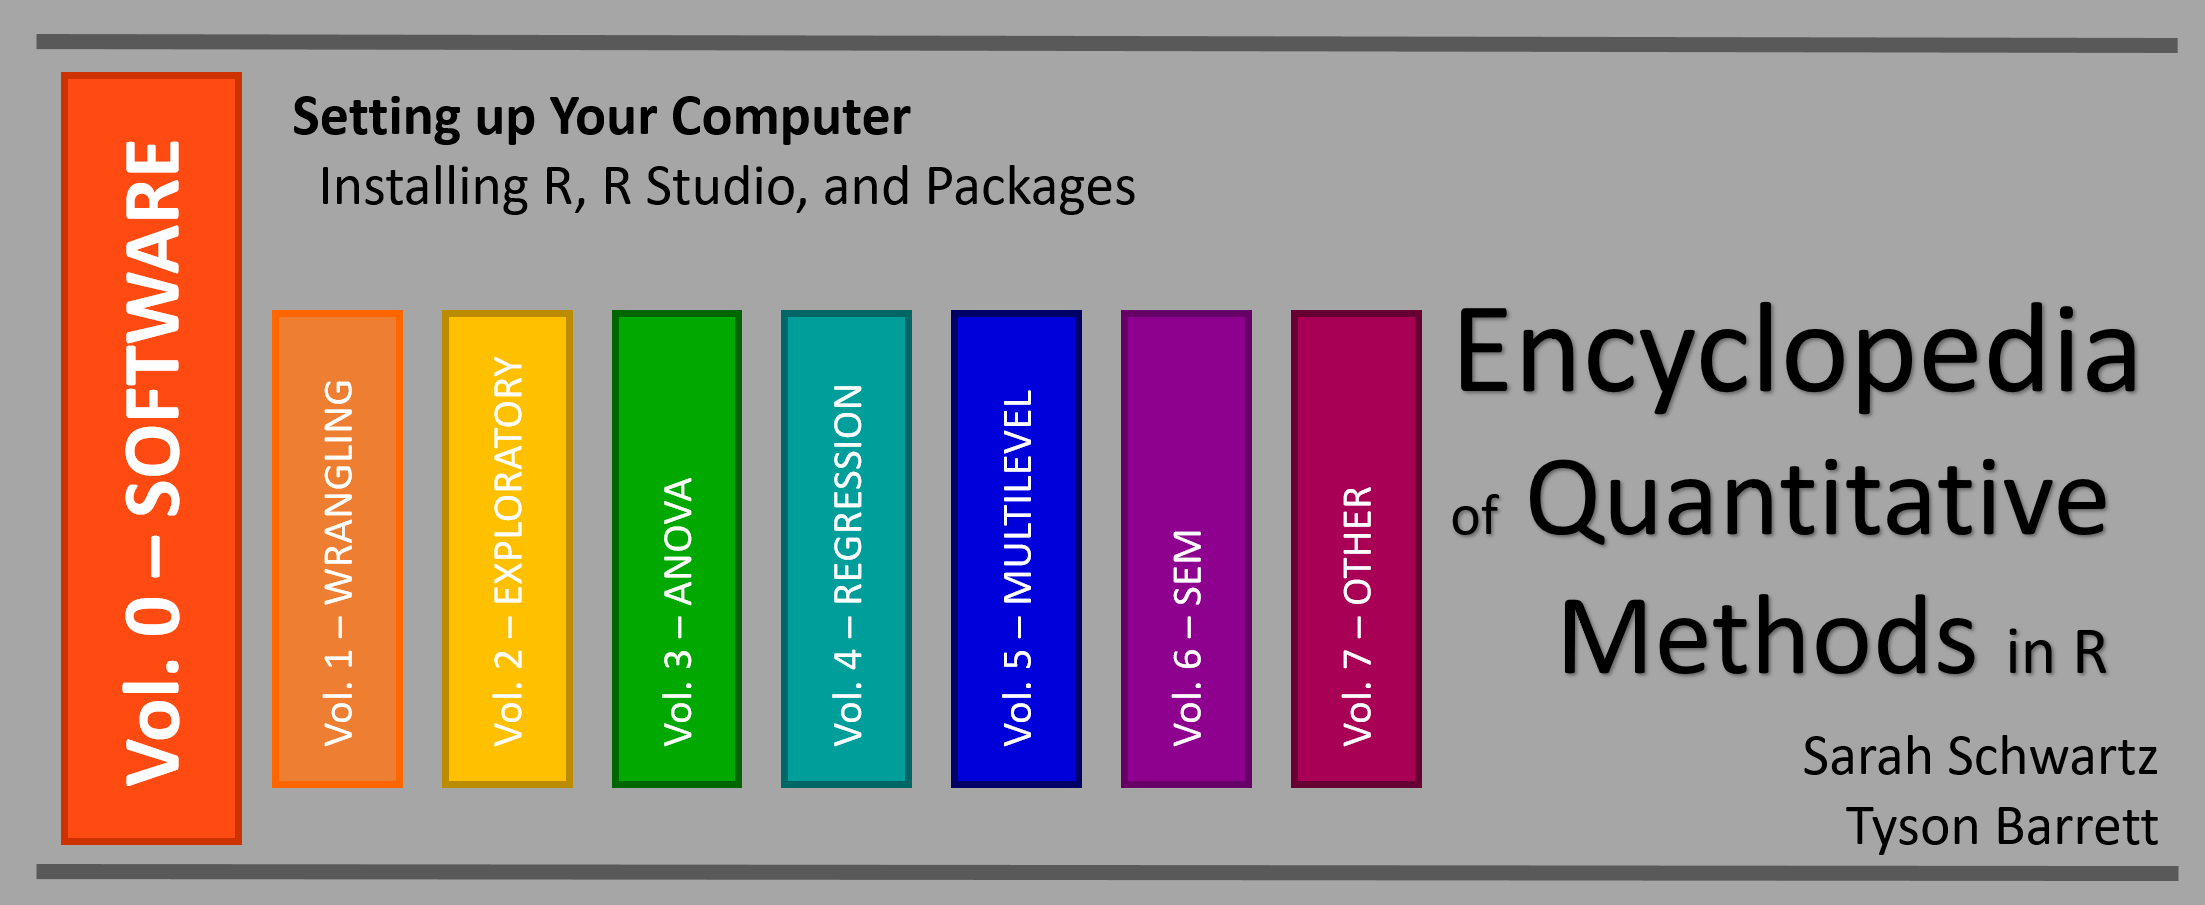
\includegraphics{images/EQM_img/EQM_v0_header.png}
\caption{}
\end{figure}

\section*{Preface}\label{preface}
\addcontentsline{toc}{section}{Preface}

This encyclopedia of eBooks is being developed by
\href{http://www.sarahschwartzstats.com/}{Sarah Schwartz} and
\href{http://tysonbarrett.com/}{Tyson Barrett}, of the
\href{https://cehs.usu.edu/research/index}{Office of Research Services},
to support faculty and graduate students in the
\href{https://cehs.usu.edu/}{College of Education and Human Services} at
\href{http://www.usu.edu/}{Utah State University}. It serves as
reference material for graduate courses (EDUC/PSY 6600, EDUC/PSY 7610,
PSY 7650, ect.), as well as college wide workshops and individualized
consultation from the
\href{https://cehs.usu.edu/research/statstudio/index}{Statistical
Consulting Studio} and the
\href{https://cehs.usu.edu/research/dsdu/index}{Data Science and
Discover Unit}.

\begin{figure}
\centering

\includegraphics{images/cehs_statstudio_dsdu.PNG}
\caption{}
\end{figure}

\begin{center}\rule{0.5\linewidth}{\linethickness}\end{center}

\section*{Background FAQs}\label{background-faqs}
\addcontentsline{toc}{section}{Background FAQs}

\subsection*{What is R ?}\label{what-is-r}
\addcontentsline{toc}{subsection}{What is R ?}

\begin{quote}
\(R\) is a language and environment for statistical computing and
graphics. \citep{R-base}
\end{quote}

\(R\) provides a wide variety of \textbf{statistical} \emph{(linear and
nonlinear modelling, classical statistical tests, time-series analysis,
classification, clustering, \ldots{})} and \textbf{graphical}
techniques, and is highly extensible. The \(S\) language is often the
vehicle of choice for research in statistical methodology, and \(R\)
provides an Open Source route to participation in that activity.

One of \(R\)'s strengths is the ease with which well-designed
publication-quality plots can be produced, including mathematical
symbols and formulae where needed. Great care has been taken over the
defaults for the minor design choices in graphics, but the user retains
full control.

\begin{center}\rule{0.5\linewidth}{\linethickness}\end{center}

\subsection*{What is R Markdown ?}\label{what-is-r-markdown}
\addcontentsline{toc}{subsection}{What is R Markdown ?}

According to \href{www.rstudio.com}{R Studio}:

\begin{quote}
``R Markdown is a format that enables easy authoring of reproducible web
reports from R. It combines the core syntax of Markdown (an
easy-to-write \emph{plain text} format for web content) with embedded
\emph{\(R\) code chunks} that are run so their output can be included in
the final document''.
\end{quote}

\begin{center}\rule{0.5\linewidth}{\linethickness}\end{center}

\subsection*{What is Dynamic
Reporting?}\label{what-is-dynamic-reporting}
\addcontentsline{toc}{subsection}{What is Dynamic Reporting?}

From
\href{https://onlinecourses.science.psu.edu/statprogram/markdown}{Penn
State Statistics}:

The traditional way to write a report:

\begin{enumerate}
\def\labelenumi{\arabic{enumi}.}
\tightlist
\item
  Run your analysis in software, like SPSS or R and manually save our
  output

  \begin{itemize}
  \tightlist
  \item
    \emph{i.e.~saving the ANOVA table or using \texttt{pdf()} to save
    the graphs}
  \end{itemize}
\item
  Type your your description and interpretation in a text editor like
  \emph{Word}

  \begin{itemize}
  \tightlist
  \item
    \emph{either drag/drop tables and figures, or worse copy-paste and
    retype all the numbers}
  \end{itemize}
\end{enumerate}

A report written in this way can be problematic. For instance, imagine
your \emph{Mentor/collaborator/journal reviewer} telling you that they
want to use a sub-sample instead of the entire sample. Or to include a
nother variable. You would have to redo all of your work!!

Therefore, in this way \textbf{dynamic also means reproducible}, in the
sense that people who get the file from you can reproduce the entire
work in the report.

\begin{center}\rule{0.5\linewidth}{\linethickness}\end{center}

\subsection*{\texorpdfstring{How does R Markdown work out to be a
\texttt{.pdf} or \texttt{.html}
file?}{How does R Markdown work out to be a .pdf or .html file?}}\label{how-does-r-markdown-work-out-to-be-a-.pdf-or-.html-file}
\addcontentsline{toc}{subsection}{How does R Markdown work out to be a
\texttt{.pdf} or \texttt{.html} file?}

\(R Markdown\) is a file with the file extension \texttt{.Rmd}, the
\texttt{knitr} package will then transform the file into a
\emph{Markdown} file with the extension \texttt{.md.} Then \(R Studio\)
can \citep{xie2015}:

\begin{itemize}
\item
  Use \(LaTeX\) to transform the file into a \texttt{.pdf}
\item
  Load another package called \(markdown\) to transform the file into
  \texttt{.html}
\item
  Use Pandoc to even convert to file to a \texttt{Word} document (ugly)
\end{itemize}

\begin{figure}
\centering
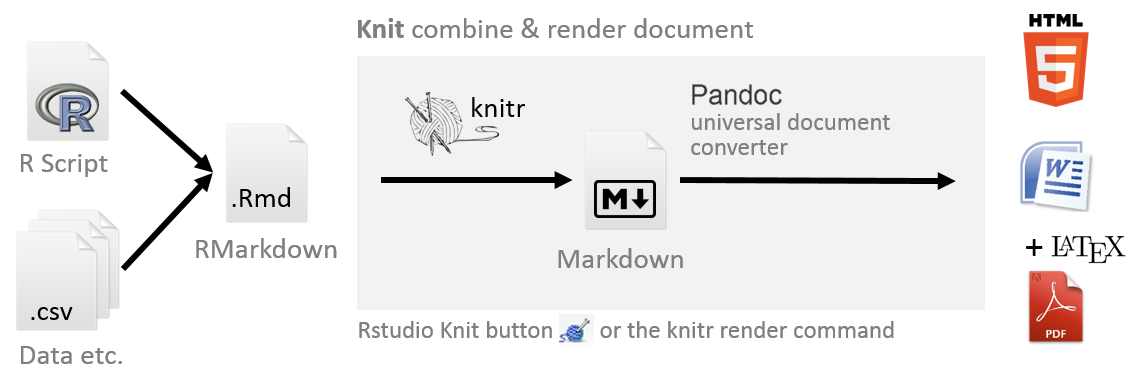
\includegraphics{images/processRStudio.png}
\caption{}
\end{figure}

The professionals ar \(R Studio\) show it better at their
\href{https://rmarkdown.rstudio.com/index.html}{website}.

\begin{center}\rule{0.5\linewidth}{\linethickness}\end{center}

\subsection*{Is this a popular method for creating
reports?}\label{is-this-a-popular-method-for-creating-reports}
\addcontentsline{toc}{subsection}{Is this a popular method for creating
reports?}

Check out \href{http://rpubs.com/}{Rpubs}. This website shares lots of
documents written in the way we will introduce below.

\chapter{An Overview}\label{an-overview}

\begin{figure}
\centering

\includegraphics{images/headers/R_studio_LaTeX_header.png}
\caption{}
\end{figure}

Before we get busy downloading and installing the actual software, here
is the big picture.

\begin{center}\rule{0.5\linewidth}{\linethickness}\end{center}

\section{R vs.~R Studio}\label{r-vs.r-studio}

First time users often confuse by all the different uses of the letter
``R''.

\begin{longtable}[]{@{}ll@{}}
\toprule
\(R\) & \(R Studio\)\tabularnewline
\midrule
\endhead
Engine & Dashboard\tabularnewline
Install and Ignore & Interact with Constantly\tabularnewline
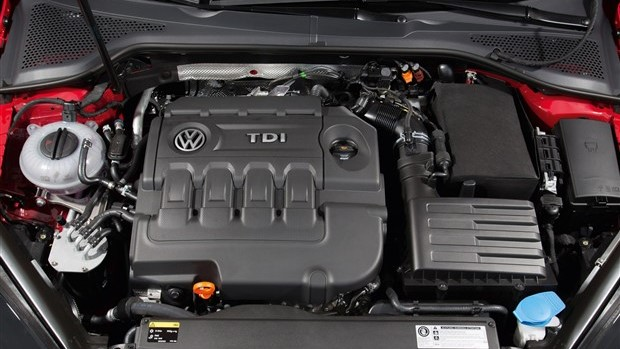
\includegraphics[width=5.20833in]{images/car_engine.jpg} &
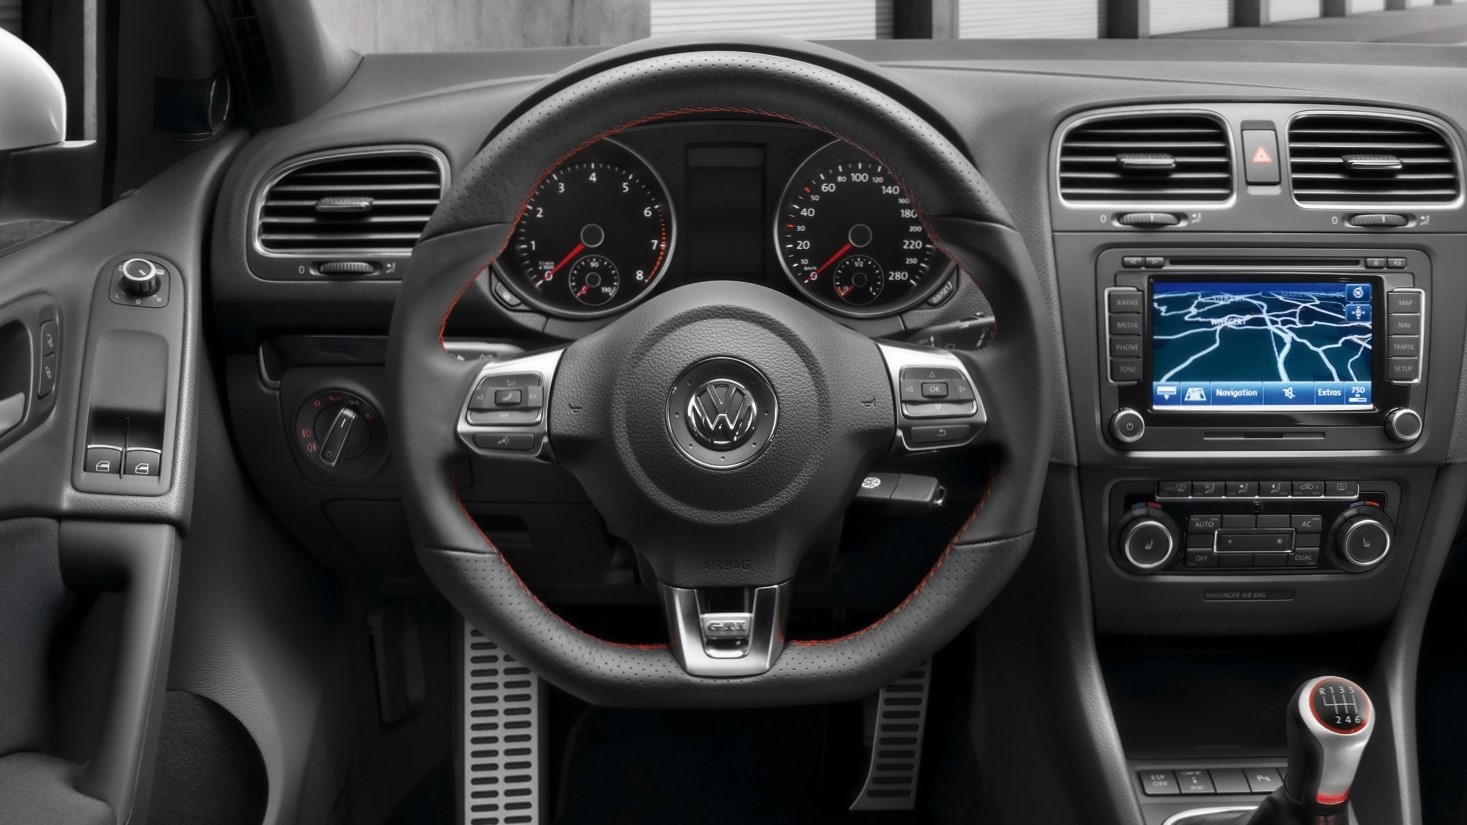
\includegraphics[width=5.20833in]{images/car_dashboard.jpg}\tabularnewline
\bottomrule
\end{longtable}

\begin{quote}
More precisely, \(R\) is a \emph{programming language} that runs
computations while \(R Studio\) is an \emph{integrated development
environment (IDE)} that provides an interface by adding many convenient
features and tools. So the way of having access to a speedometer,
rearview mirrors, and a navigation system makes driving much easier,
using \(RStudio’s\) interface makes using \(R\) much easier as well. -
\href{https://ismayc.github.io/moderndive/index.html}{Chester Ismay and
Albert Y. Kim}
\end{quote}

\begin{rmdtip}
For a more in-depth discussion on the difference between \(R\) and
\(R Studio\) IDE, watch this
\href{https://campus.datacamp.com/courses/working-with-the-rstudio-ide-part-1/orientation?ex=1}{DataCamp
video (2m52s)}.
\end{rmdtip}

\begin{center}\rule{0.5\linewidth}{\linethickness}\end{center}

\section{R Markdown vs.~R Notebook}\label{r-markdown-vs.r-notebook}

\begin{center}\rule{0.5\linewidth}{\linethickness}\end{center}

\section{The Magic of Knit'ing}\label{the-magic-of-kniting}

\begin{figure}
\centering

\includegraphics{images/hex/rmarkdown-200x232.png}
\caption{}
\end{figure}

\begin{quote}
\(R Markdown\) documents are fully reproducible. Use a productive
\textbf{notebook} interface to weave together narrative text and code to
produce elegantly formatted output. Use multiple languages including
\(R\), \(Python\), and \(SQL\) \citep{R-rmarkdown}.
\end{quote}

\begin{figure}
\centering

\includegraphics{images/hex/knitr-200x232.png}
\caption{}
\end{figure}

\begin{quote}
\texttt{knitr} is an engine for dynamic report generation with \(R\). It
is a package in the statistical programming language \(R\) that enables
integration of \textbf{R code} into \(LaTeX\), \(LyX\), \(HTML\),
\(Markdown\), \(AsciiDoc\), and \(text\)s documents \citep{R-knitr}.
\end{quote}

\begin{center}\rule{0.5\linewidth}{\linethickness}\end{center}

\begin{rmdtip}
Helpful Website:
\href{https://www.statmethods.net/stats/index.html}{Quick R: Basic
Statistics}
\end{rmdtip}

\chapter{Install R}\label{install-r}

\begin{figure}
\centering

\includegraphics{images/Rlogo_200.png}
\caption{}
\end{figure}

Here is where we talk about installing R.

\begin{center}\rule{0.5\linewidth}{\linethickness}\end{center}

\section{First Time Installation}\label{first-time-installation}

\begin{quote}
Go to: \href{http://www.r-project.org}{www.r-project.org}
\end{quote}

Get the latest released version of FREE \textbf{Base} \(R\) from
\(CRAN\)

\begin{itemize}
\tightlist
\item
  Choose a mirror close to your geographical location
\item
  Select \textbf{base} \(R\) for your computer \emph{(Windows, Mac,
  ect.)}
\item
  The defaults are good\ldots{}don't change them\ldots{}just keep
  clicking \emph{`Next'}
\end{itemize}

\begin{center}\rule{0.5\linewidth}{\linethickness}\end{center}

\section{Update Regularly}\label{update-regularly}

\chapter{Install R Studio}\label{install-r-studio}

\begin{figure}
\centering

\includegraphics{images/rstudiosticker.png}
\caption{}
\end{figure}

Here is where we talk about installing R Studio.

\begin{center}\rule{0.5\linewidth}{\linethickness}\end{center}

\section{First Time Installation}\label{first-time-installation-1}

\begin{quote}
Go to: \href{http://www.rstudio.com}{www.rstudio.com}
\end{quote}

Get the latest version of the FREE Open Source \textbf{Desktop} Edition
of R Studio

\begin{itemize}
\tightlist
\item
  The defaults are good\ldots{}don't change them\ldots{}just keep
  clicking \emph{`Next'}
\end{itemize}

\begin{center}\rule{0.5\linewidth}{\linethickness}\end{center}

\section{Update Regularly}\label{update-regularly-1}

\begin{center}\rule{0.5\linewidth}{\linethickness}\end{center}

\section{Panel Layout}\label{panel-layout}

\chapter{Install TeX}\label{install-tex}

\begin{figure}
\centering

\includegraphics{images/latex.png}
\caption{}
\end{figure}

Here is where we talk about installing Tex.

\begin{center}\rule{0.5\linewidth}{\linethickness}\end{center}

\section{\texorpdfstring{Use \texttt{tinytex}
package}{Use tinytex package}}\label{use-tinytex-package}

\begin{center}\rule{0.5\linewidth}{\linethickness}\end{center}

\section{\texorpdfstring{Mac - use
\texttt{MacTeX}}{Mac - use MacTeX}}\label{mac---use-mactex}

\begin{quote}
Go to: \url{http://tug.org/mactex/}
\end{quote}

\begin{itemize}
\tightlist
\item
  Download (5+ min) to a folder and them double click on the \textbf{PKG
  file}
\item
  Follow the installation instructions.
\item
  You don't need to open anything after MacTeX is finished installing.
\end{itemize}

\begin{center}\rule{0.5\linewidth}{\linethickness}\end{center}

\section{\texorpdfstring{Windows - use
\texttt{MikTeX}}{Windows - use MikTeX}}\label{windows---use-miktex}

\begin{quote}
Go to: \url{http://miktex.org/download}
\end{quote}

\begin{itemize}
\tightlist
\item
  Pick the latest version of the \textbf{Net Installer}, not the Basic!
\item
  You need the full version 64-bit is better, if you have a 64-bit
  machine
\item
  When your download is complete, run the downloaded installer.
\item
  Windows may ask you if you want to \emph{``allow this app from an
  unknown publisher to make changes to your PC''}. If it does, make sure
  to click \textbf{Yes!}
\item
  This is the slowest part\ldots{}
\end{itemize}

\chapter{Install Packages}\label{install-packages}

We describe packages and their management

\begin{center}\rule{0.5\linewidth}{\linethickness}\end{center}

\section{What are packages}\label{what-are-packages}

\begin{quote}
\textbf{R packages} are collections of functions and data sets developed
by the community. They increase the power of \textbf{R} by improving
existing base \textbf{R} functionalities, or by adding new ones.
\end{quote}

More information may be found here:
\url{https://www.datacamp.com/community/tutorials/r-packages-guide}

\begin{center}\rule{0.5\linewidth}{\linethickness}\end{center}

\section{Installing packages (via the user
interface)}\label{installing-packages-via-the-user-interface}

\begin{quote}
You only need to INSTALL packages ONCE per computer.
\end{quote}

In \textbf{R Stuido}:

\begin{enumerate}
\def\labelenumi{\arabic{enumi}.}
\tightlist
\item
  Click on the \textbf{Packages} tab the panel with the most tabs
\item
  Click on the word \textbf{Instsall} just under and to the left of the
  tab
\item
  In the \textbf{Packages} box, type in the name of the packages you
  would like to download. You can do several at once, just seperate them
  with multiple spaces or a comma.
\end{enumerate}

\emph{Note: Leave the installation library path as the default. Also,
make sure the box for `Installing dependencies' is checked.}

\begin{figure}
\centering
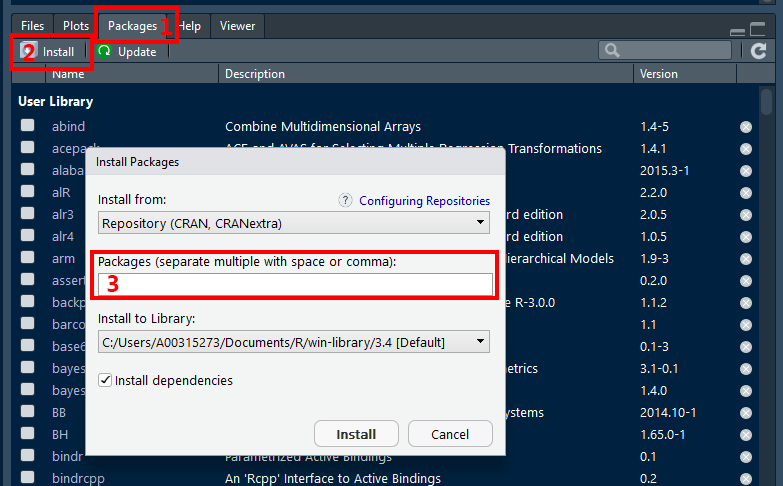
\includegraphics{images/Install_Package_Screenshot.png}
\caption{}
\end{figure}

You can \emph{copy-and-paste} the following list into the box (labeled
3) to load the packages that we use most commonly all at once.

\begin{quote}
tidyverse, furniture, pander, stargazer, texreg, xtable, RColorBrewer,
gghighlight, ggthemes, ggfortify, ggalt, ggExtra, GGally, ggeffects,
corrplot, gpairs, gridextra, likert, vcd, scales, cowplot, yarrr, psych,
polycor, corpcor, sjlabelled, sjPlot, sjmisc, sjstats, Hmisc, labelled,
afex, emmeans, corpcor, multicomp, multcompView, car, effects,
predictmean, nlme, lme4, lmerTest, HLMdiag, geepack, gee, gee4, optimx,
MuMIn, lavaan, OpenMx, sem, semPlot, randomForest, randomForestSRC,
ggRandomForests, party, partykit, mgcv, glmnet, survival, caret,
bookdown, blogdown, tidytex, xaringan, REDCapR, redcapAPI, devtools,
testthat, roxygen2
\end{quote}

When you click the \textbf{Install} buttom, a smaller window may asks if
you would like to re-start \(R\) prior to installing, choose ``no'' and
manually close and open the \(R Studio\) program once all packages have
been downloaded, unpacked, and checked. This may take a few minutes,
especially if you have selected multiple packages.

\begin{quote}
See Chapter 6 for more information on how to install packages another
way (via syntax code), as well as website links for each package.
\end{quote}

\begin{center}\rule{0.5\linewidth}{\linethickness}\end{center}

\section{Updating packages}\label{updating-packages}

\chapter{Kniting Notebooks}\label{kniting-notebooks}

\begin{center}\rule{0.5\linewidth}{\linethickness}\end{center}

\section{Storing all associated
files}\label{storing-all-associated-files}

If you are using any files, such as \emph{datasets} or \emph{images},
they need to be stored in the same folder location as the R Notebook
(\texttt{.Rmd} file).

This folder location must be the \textbf{Working Directory} for the R
Studio session. If you opened your \texttt{.Rmd} notebook file by
double-clicking on its name, then this should be the case.

\begin{center}\rule{0.5\linewidth}{\linethickness}\end{center}

\section{Setting the working
directory}\label{setting-the-working-directory}

To ensure that R Studio knows where to find the files, you can manually
set the \textbf{Working Directory} through the menu:

\begin{itemize}
\tightlist
\item
  Click \texttt{Session}
\item
  Select \texttt{Set\ Working\ Directory} by hovering your mouse over it
\item
  Click on \texttt{To\ Source\ File\ Location}
\end{itemize}

\begin{figure}
\centering
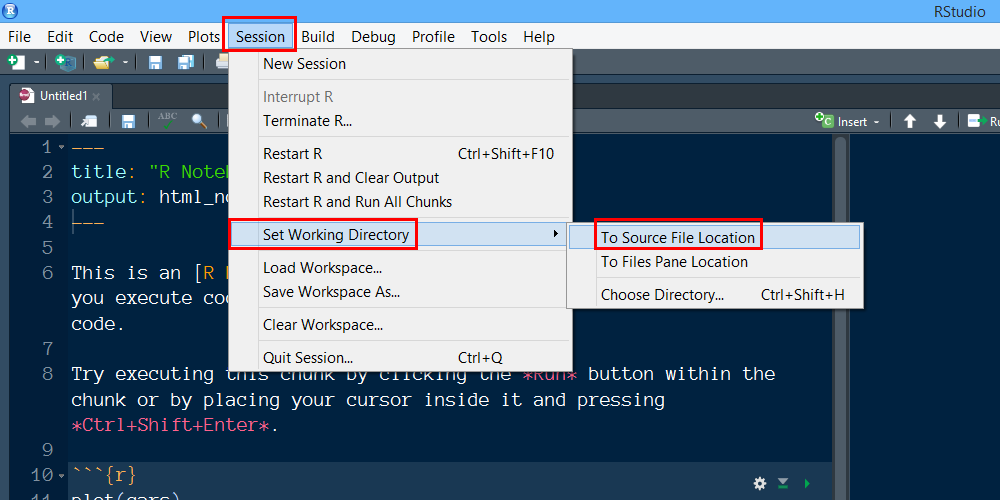
\includegraphics{images/Set_wd_source.png}
\caption{}
\end{figure}

You can double check that you were successful by

\begin{itemize}
\tightlist
\item
  Click on the \texttt{Files} tab in the many-tab panel
\item
  Click on the button with the gear that says \texttt{More}
\item
  Click \texttt{Go\ To\ Working\ Directory}
\end{itemize}

At this point you should see all the files that reside in the folder
location where the open \texttt{.Rmd} files is also saved.

\begin{figure}
\centering
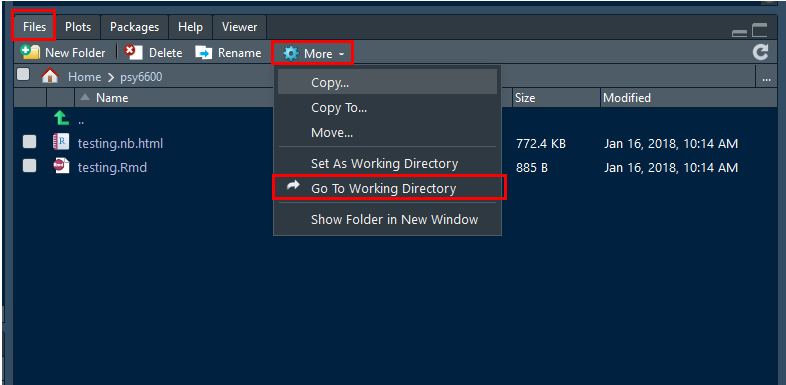
\includegraphics{images/files_goto_wd.png}
\caption{}
\end{figure}

\begin{center}\rule{0.5\linewidth}{\linethickness}\end{center}

\section{Press the Knit button}\label{press-the-knit-button}

\bibliography{book.bib,packages.bib}


\end{document}
